\section*{\centering BAB V \\ Hasil Implementasi }

\addcontentsline{toc}{section}{BAB V Hasil Implementasi}  % Manually add unnumbered section to ToC

% Set the section counter manually to "1" for subsections under BAB IV
\setcounter{section}{5}
\setcounter{subsection}{0}  % Reset subsection
\setcounter{figure}{0}
\setcounter{table}{0}
\setcounter{lstlisting}{0}
\renewcommand{\thetable}{\thesection.\arabic{table}}
\renewcommand{\thefigure}{\thesection.\arabic{figure}}
\renewcommand{\thelstlisting}{\thesection.\arabic{lstlisting}}

\subsection{Data Preparation}
Dalam penelitian ini, digunakan dataset rekapitulasi daftar pemilih dan data tambahan dari BPS untuk menambah wawasan tentang visualisasi yang dilakukan. Dataset disimpan di dalam file csv untuk memudahkan pemrosesan data tahap lanjut.
\begin{table}[ht]
\centering
\resizebox{\textwidth}{!}{
\begin{tabular}{|l|r|r|r|r|r|r|r|r|}
\hline
\textbf{Sub-Region} & \textbf{Male Voters} & \textbf{Female Voters} & \textbf{Total Voters} & \textbf{Voter Gender Ratio} & \textbf{Total Population} & \textbf{Population Growth Rate (\%)} & \textbf{Population Density} & \textbf{Eligible Voter Ratio} \\ \hline
KEDATON             & 19196                & 19657                 & 38853                & 97.65                      & 52400                    & -0.17                              & 13896                      & 74.146947                      \\ \hline
SUKARAME            & 23913                & 24623                 & 48536                & 97.12                      & 67100                    & 0.65                               & 6148                       & 72.333830                      \\ \hline
TANJUNG KARANG BARAT & 22329                & 22631                 & 44960                & 98.67                      & 63200                    & 0.72                               & 5476                       & 71.139241                      \\ \hline
PANJANG             & 26859                & 26298                 & 53157                & 102.13                     & 74900                    & 0.23                               & 5488                       & 70.970628                      \\ \hline
TANJUNG KARANG TIMUR & 14017                & 14236                 & 28253                & 98.46                      & 38500                    & -0.37                              & 18619                      & 73.384416                      \\ \hline
\end{tabular}
}
\caption{Dataset Rekapitulasi Daftar Pemilih}
\label{tab:voter_population_data}
\end{table}

\subsection{Data Preprocessing}
Tahap \textit{Preprocessing} merupakan tahapan dimana data yang telah diambil sebelumnya akan dilakukan pengolahan lebih lanjut sebelum digunakan sebagai data untuk proses clustering. Bisa dilihat dari table \ref{tab:voter_population_data} terdapat beberapa data mentah seperti jumlah pemilih laki-laki dan perempuan, maka dibuat atribut data baru \textit{Voters Gender Ratio} sebagai atribut data baru dari kedua ata sebelumya untuk memudahkan analisis. Hasil akhir yang digunakan adalah 4 atribut data berupa \textit{Eligible Voter Ratio}, \textit{Voter Gender Ratio}, \textit{Kepadatan Penduduk} dan \textit{Percentase Pertumbuhan Penduduk}

\subsection{Model Building}
Akan dibuat model clustering dan proses visualisasi dari 4 atribut ini dari berbagai macam sudut pandang, namun hal peratama yang perlu dilakukan adalah menentukan jumlah \textit{cluster} yang sesuai untuk dataset kali ini.

\begin{lstlisting}[language=Python, caption=Python Code for Elbow Methods,label={lst:elbow_method}]
## Install the Necessary Package
import numpy as np
import pandas as pd
import matplotlib.pyplot as plt

## Open and read the csv data
file_path = "dataset-rekapitulasi-dpt-kecamatan.csv"
df = pd.read_csv(file_path)

# Display the first few rows to understand the structure
df.head()

# Select the features for clustering
data = df[['Eligible Voter Ratio', 'Population Growth Rate (%)', 'Population Density', 'Voter Gender Ratio']]

# Normalize the data
scaler = StandardScaler()
data_scaled = scaler.fit_transform(data)

# Perform KMeans can calculate SSE (Sum Squared Error) for K values
sse = []
K_range = range(1, 10)

for k in K_range:
    kmeans = KMeans(n_clusters=k, random_state=17)
    kmeans.fit(data_scaled)
    sse.append(kmeans.inertia_)

# Plot Elbow Method
fig, ax = plt.subplots(figsize=(8, 5))
ax.plot(K_range, sse, marker='o')
ax.set_xlabel('Number of Clusters')
ax.set_ylabel('SSE (Sum of Squared Errors)')
ax.set_title('Elbow Method for Optimal K')
plt.show()
\end{lstlisting}

\begin{figure}[h]
    \centering
    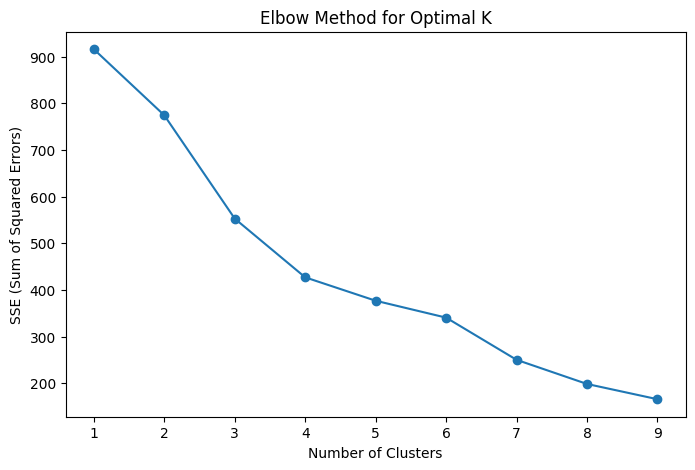
\includegraphics[width=0.5\linewidth]{images/optimum_cluster.png}
    \caption{Hasil Elbow Method}
    \label{fig:elbow_method}
\end{figure}

Berdasarkan hasil tersebut didapatkan bahwa nilai kluster yang optimal adalah 4, dimana setelah cluster ke-4 grafik tersebut menjadi lebih landai.

\subsection{Analisis}
Hasil dari \textit{Model Building} dan ketika dilakukan klusterisasi data rekapitulasi daftar pemilih, disini akan dijelaskan tentang hasil analisis dari masing-masing visualisasi.

\subsubsection{Pair Plot Analysis}
Metode analisis yang membandingkan nilai dari masing-masing atribute dan melihat sifat alami dari atribut data tersebut.
\begin{figure}[h]
    \centering
    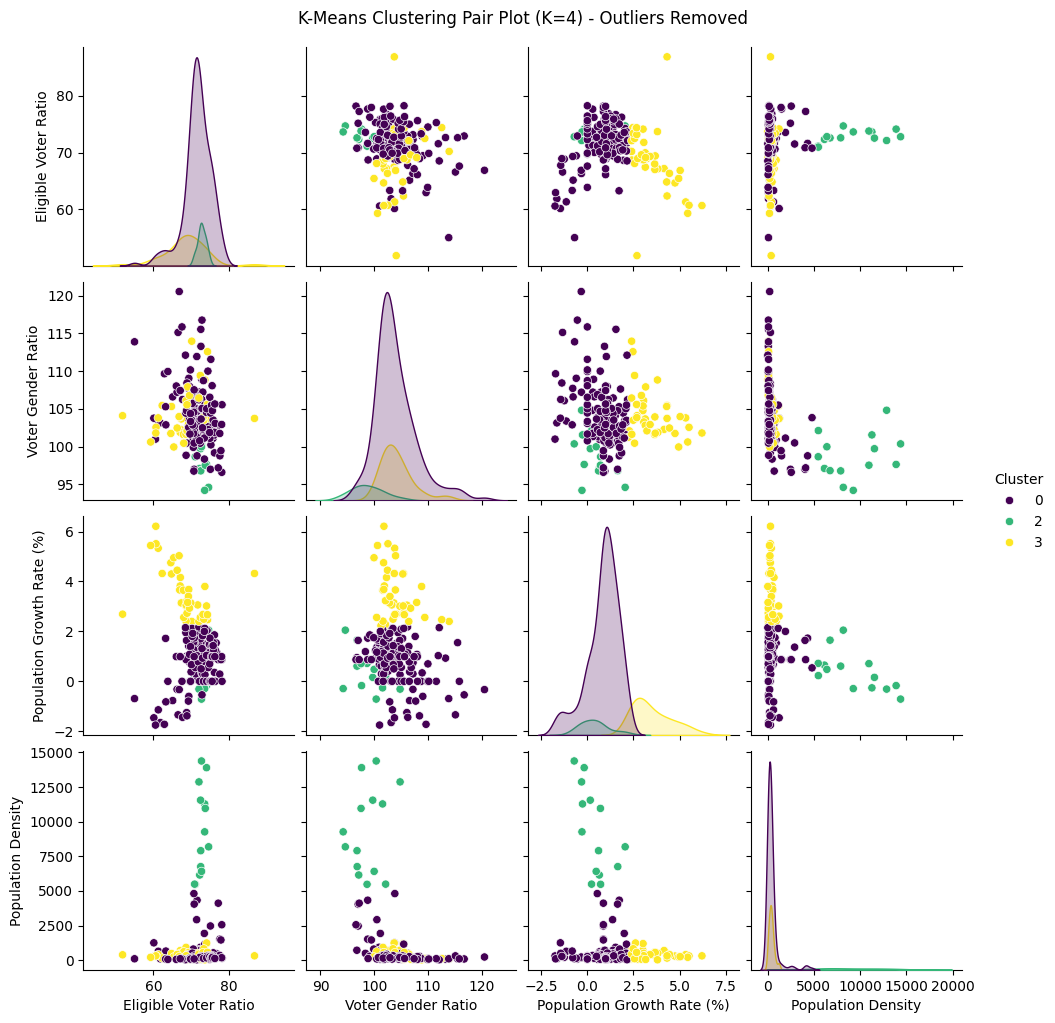
\includegraphics[width=1\linewidth]{images/pair_plot_analysis.png}
    \caption{Hasil Pair Plot}
    \label{fig:pair_plot}
\end{figure}
Hasil analisis dari \ref{fig:pair_plot} menunjukan bahwa interaksi antar atribut data, dari visualisasi ini juga didapatkan bahawa terdapat homogenitas serta kurangnya standar deviasi (persebaran data) dalam beberapa atribut data sehingga didapatkan grafik yang tumpang-tindih (\textit{overlapped}).

\subsubsection{3d Visualization Analysis}
Metode visualisasi dengan menggunakan visualisasi 3 dimensi untuk mendapatkan perspektif baru dari penelitian ini.

\begin{figure}[h]
\begin{subfigure}{0.5\textwidth}
    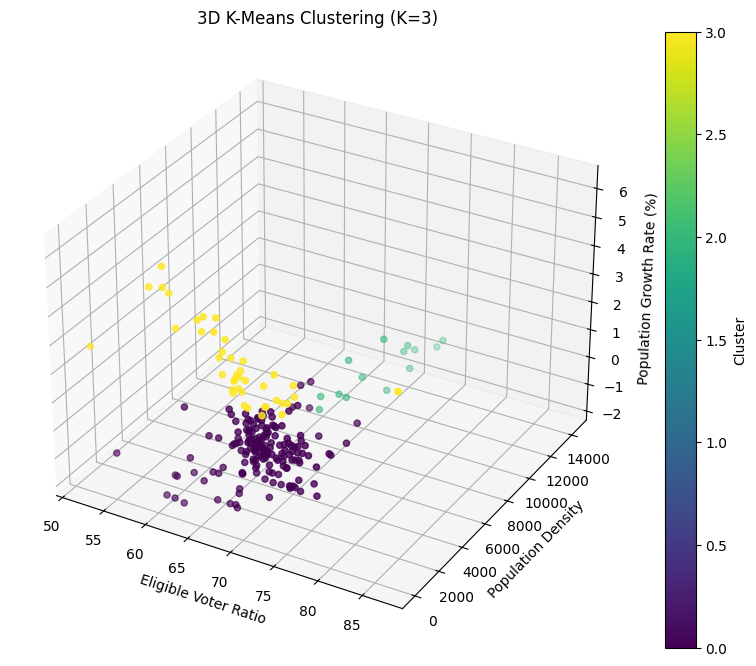
\includegraphics[width=1\linewidth]{images/first_3d_visual.png}
    \caption{First 3D Visualization}
    \label{fig:first_3d_visual}

\end{subfigure}
\begin{subfigure}{0.5\textwidth}
        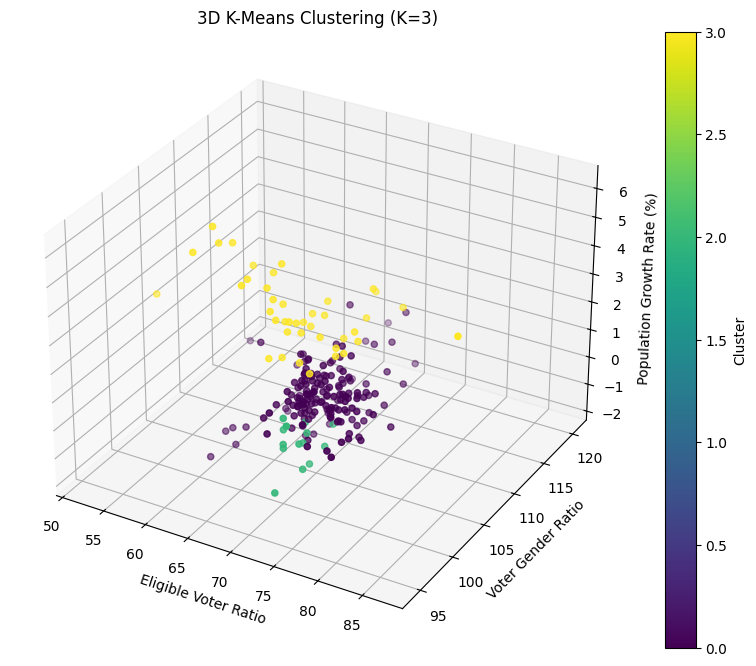
\includegraphics[width=1\linewidth]{images/second_3d_visual.png}
    \caption{Second 3D Visualization}
    \label{fig:second_3d_visual}

\end{subfigure}
\begin{subfigure}{1\textwidth}
    \centering
    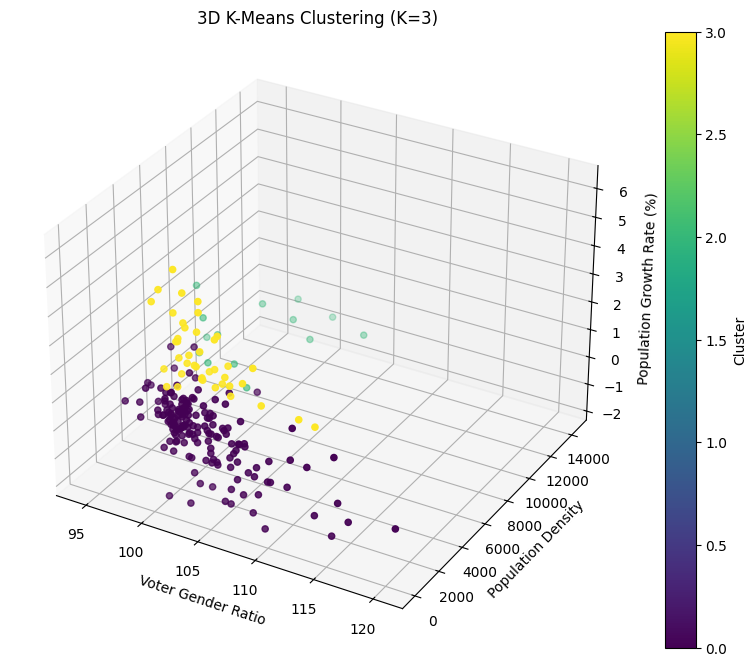
\includegraphics[width=0.5\linewidth]{images/third_3d_visual.png}
    \caption{Third 3D Visualization}
    \label{fig:third_3d_visual}
\end{subfigure}

    \caption{3D Visualization}
    \label{fig:3d_visual}

\end{figure}

Pada visualisasi ini didapatkan hasil bahwa visualisasi 3D memberikan hasil yang lebih baik dibandingkan dengan \textit{Pair Plot analysis}. Namun karena sifat alami dari data tersebut, masih terdapatnya Homogenitas data, dimana atribut data \textit{voter ratio} dan \textit{voter gender ratio, } menunjukan adanya keterkaitan antar dua atribut sehingga data tersebut saling tumpang-tindih \textit{overlap}.

\subsubsection{PCA Analysis}
Secara keseluruhan, proyeksi PCA ini menunjukkan bahwa Cluster 0 dan 1 tidak mudah dipisahkan dan memiliki tumpang tindih yang cukup besar, yang memperkuat homogenitas data dalam atribut tertentu. Variansi lebih banyak tertangkap pada Komponen Utama 1, yang kemungkinan dipengaruhi oleh atribut dengan variansi lebih tinggi seperti Tingkat Pertumbuhan Populasi dan Kepadatan Populasi, sementara Komponen Utama 2 tidak berkontribusi banyak pada pemisahan cluster.
\begin{figure}[H]
    \centering
    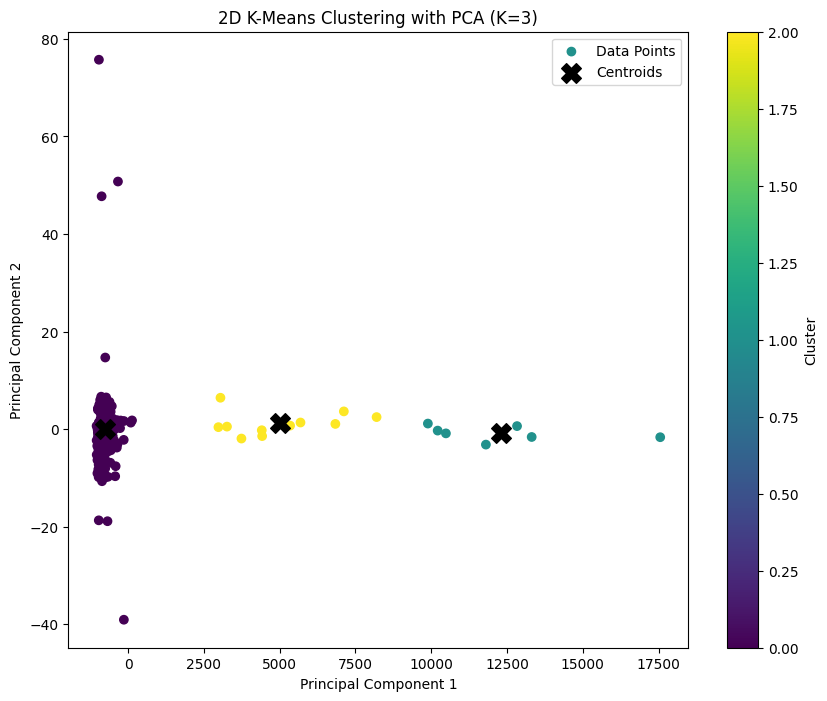
\includegraphics[width=0.5\linewidth]{images/pca_visual.png}
    \caption{PCA Analysis}
    \label{fig:pca_analysis}

\end{figure}
\newpage

